\documentclass[9pt,twocolumn,twoside]{idsi}
% Defines a new command for the horizontal lines, change thickness here
\newcommand{\HRule}{\rule{\linewidth}{0.5mm}} 
\usepackage{listings}
\renewcommand{\headrulewidth}{2pt}
\fancypagestyle{plain}{%
  \fancyhead[L]{
    \begin{tabular}{ll}
%        
\includegraphics[scale=0.15]{figs/ncsa_vertical} 
    \end{tabular}
  }
  \fancyhead[C]{
      	\begin{tabular}[m]{c}
		  	\fontsize{20}{20} Illinois Data Science Initiative    	
		\end{tabular}
  }

  \fancyhead[R]{
    \begin{tabular}{ll}
%	  	
\includegraphics[scale=0.125]{figs/ill}  		
  	\end{tabular}
  }
  
  \fancyfoot[C]{\thepage}
}
\pagestyle{plain}
\def \report_title { Comparing Credit Card Fraud Detection between Spark and Spark Streaming   }
\author[1]{Arshia Malkani, Caren Zeng}
\author[2]{Professor Robert J. Brunner}
\affil[1]{National Center For Supercomputing Applications (NCSA)}
\affil[2]{Laboratory for Computation, Data, and Machine Learning}
\title{Comparing Credit Card Fraud Detection between Spark and Spark Streaming}

\begin{abstract}

\end{abstract}

\begin{document}

\coverpage{Comparing Credit Card Fraud Detection between Spark and Spark Streaming}{Arshia Malkani, Caren Zeng}

\maketitle

\section{Introduction}
Different classification methods on Spark yield comparable results as the formulaic construction of such methods are similar. However, the pipelining process for Spark Streaming has the potential to analyze and run machine learning algorithms and yield more interesting classification results. We wanted to analyze both the efficiency and accuracy of spark vs spark streaming for machine learning on credit card fraud data.  

\section{The Data}
Our goal was to predict credit card fraud detection by using Logistic Regression, Linear Support Vector Machines (SVMs), and K-means classification on one dataset. The dataset we used is a 68.08MB CSV of anonymized credit card data, including features such as the frequency of usage of the card, the transaction amount, and a binary value indicating fraud (“1”) or non-fraud (“0”).

The main features we chose to utilize are the transaction amount and the binary indicator of fraud. We recognize that utilizing other features of data like frequency of usage of the card, credit score, and distance between the usage and the credit card holder’s home address would allow us to create a more accurate model for predicting fraud, but to develop a more complicated model involves deeper research into deciding appropriate weight ages for each feature, beyond the scope and tangent to the purpose of this paper. This is grounds for expansion upon this report, if provided more time.

Before developing algorithms to predict features of our data, we analyzed our data to understand what its characteristics were and how they would influence building our models and how reliable each should be considered. Running a percentage-generating script on our dataset, it was apparent that the dataset was very unbalanced, with only 0.173 of our data labeled as fraud. This skews our models as a precondition to build an accurate model is a balanced dataset. This feature also yielded atypical results in our Linear and Logistic Regressions, as documented in further sections.  

In order to clean the csv file, we mapped and filtered the data to remove the first line and turn the columns containing the amount of money spent, number of times the card was used, and whether not it was fraud into a labeled point. This format would allow use to run the machine learning algorithms necessary in spark. 
\begin{verbatim}

def clean(x):
    if (x[29] != "Amount"):
        return x
        
def normalize(x):
    return LabeledPoint(float(x[30]), 
    	[float(x[0]), float(x[29])/ 25691.16])

rdd = sc.textFile("creditcard.csv")
data = rdd.mapPartitions(lambda x: csv.reader(x))
data = data.map( lambda x: clean(x) )
data = data.filter(lambda x: x != None)
normalizedData = data.map(normalize)

(trainingData, testData) = 
      normalizedData.randomSplit([0.7, 0.3]) 
 \end{verbatim}

\section{Spark: Logistic Regression}
Logistic regression is a predictive regression analysis that fits the data points as if they are along a continuous function.  It is used to explain the relationship between one dependent binary variable and one or more nominal, ordinal, interval or ratio-level independent variables. In our case, the ordinal independent variables would be the purchase amount and the dependant would be the binary classification of whether or not it was fraud.  Based on the data, it tries to draw a best-fit function which is used to predict. 

We divided our dataset 70-30 into a training and test dataset and got a training error of 0.00223. We also noticed that when we accounted for both the number of times the credit card was used and the amount of money spent, the data was slightly more innaccurate that if we just accounted for the amount of money spent. This hinted that the correlation between the number of times the card was used and whether or not it was credit card fraud wasn’t that high of a correlation. 
\begin{verbatim}
lr = LogisticRegressionWithLBFGS.train(trainingData)

labelsAndPreds = testData.map(lambda p: 
      (p.label, p.features, lr.predict(p.features)))
      
trainErr = labelsAndPreds.filter(lambda d: d[0] != 
      d[2]).count() /float(testsample.count())

\end{verbatim}

Running the script multiple times yielded a consistent Training Error of 0.002 even though the data is being split differently every time, which shows the algorithm is able to consistent.


\section{Spark: Linear Support Vector Machine}
Linear SVM’s algorithm plots the data point in the n-th dimension depending on how many variables we give it, and then fits a function(hyperplane) to separate the classes of data. The function it generates tries to maximize the space between the two classes, finding the widest margin. It tends to be inaccurately predict data points near the decision boundary, which can be an issue if the data is all grouped at the boundary. We divided our dataset 70-30 into a training and test dataset and got a training error of 0.21026. The error came from the data points sitting on the decision boundary, which makes sense as we only accounted for how many times the card was used and the amount of money spent. 

\begin{verbatim}

model = SVMWithSGD.train(sample, iterations=100)

labelsAndPreds = testsample.map(lambda p: 
			(p.label, p.features, model.predict(p.features)))
            
trainErr = labelsAndPreds.filter( lambda d: 
			d[0] != d[2]).count() / float(testsample.count())
\end{verbatim}


\section{Spark: Gradient-Boosted Trees}
Gradient Boosted trees (GBTs) is a regression method for categorical features that iteratively trains decision trees to minimize a loss function. Each iteration predicts the label of each training instance then and then compares the predicted label with the true label. Before the next iteration, the dataset is relabeled to put more emphasis on training instances that yield poor predictions. These can be considered as “focus areas”, although through more iterations, gradient boosted trees may start to overfit data. This phenomena can be explained as GBTs are based off shallow decision trees, which tend to have high bias and low variance. Error is minimized by reducing both bias and variance by aggregating output from many trained models. 

While building the model, training on iterations of trees continues until the improvement of the validation error (correctness of the model) is less than a certain tolerance generated in the Boosting Strategy method.  On occasion, validation error generally decreased then later increases with more training; we did not examine the validation curve as we assumed that with an imbalanced dataset, the validation error will be strictly decreasing. 
After building our model, we attained a validation/test error of 0.0023, calculated by the formula: error = bias + variance.


\begin{verbatim}
model = GradientBoostedTrees.trainClassifier(
		trainingData,categoricalFeaturesInfo={},numIterations=3)

predictions = model.predict(testData.map
      (lambda x: x.features)) 
      
labelsAndPredictions = testData.map(lambda lp:
        lp.label).zip(predictions)
        
testErr = labelsAndPredictions.filter(lambda d: d[0] 
		!= d[1]).count()/ float(testData.count())
\end{verbatim}
\section{Spark: Random Forests }
Random forests works as a large collection of decorrelated decisions trees. Unlike Gradient-Boosted Trees (GBTs), random forests combines many decisions trees in order to reduce the risk of overfitting; such trees can be called fully grown decision trees, which provide low bias and high variance.  

It trains a set of decision trees separately, so the training can be done in parallel. The algorithm injects randomness into the training process so that each decision tree is a bit different, meaning high variance in training data but collectively resulting in low variance of error levels. Randomness is achieved by subsampling the original dataset on each iteration to get a different training set each time. However, training for decision trees is done in the same way as for individual decision trees outside of this algorithm. 

After building the model, we made predictions by aggregating the individual trees’ predictions and classifying using majority vote. The label for each test point is then predicted to be the class that receives the most votes. Our test error was calculated to be 0.00198.
\begin{verbatim}
model = RandomForest.trainClassifier(trainingData, 
		numClasses=2,categoricalFeaturesInfo={},
        numTrees=3,featureSubsetStrategy="auto",
        impurity='gini', maxDepth=4, maxBins=32)

predictions = model.predict
		(testData.map(lambda x: x.features))
        
labelsAndPredictions = testData.map
			(lambda lp:lp.label).zip(predictions)

testErr = labelsAndPredictions.filter(lambda d: d[0] 
			!= d[1]).count() / float(testData.count())
\end{verbatim}
\section{Spark: K Means }
K-Means is a clustering algorithm that tries to group data together by choosing k-number of centroids and then using euclidean distance to predict which cluster each data point fits into. For the credit card data, we divided the data into two clusters: high and low risk of fraud and graphed the data to see accurate it was. 

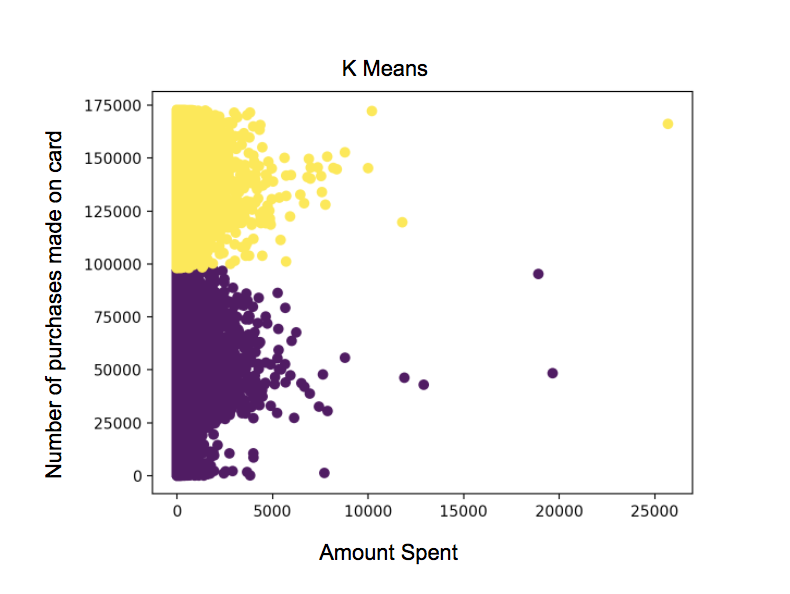
\includegraphics[scale=0.6]{two.png}

While K-means is an extremely efficient algorithm as it runs in O(n), which is significantly faster that other clustering algorithms, it is best suited to data that fits in hyper-spherical clusters and data that is evenly distributed. Due to the nature of credit card data though, the data tends to be unbalanced as there are fewer instances of fraud. For instance, in our data set , only 492 of the 284807 data points were fraud. 

\section{Spark Streams}
Spark normally runs through all the data and stores it in an RDD object. Every time a map, reduce, filter, or any other function is called, it loops through the entire RDD object and applies the operation. The difference with spark streaming though, the data is treated like a stream, so all the data isn't processed at once. The data is instead stored in a DStream, which is a sequence of RDD objects. To do this, a streaming context is initialized, which is the main entry point for all streaming functionality. 

We can see what's in the stream  through a socket running on localhost on the same port. Dstreams have functions such as map, filter, count, reduce, etc to clean the data into the format needed. It does this using windowed computation, in which the transformation is applied to a sliding window of data. In the picture below the window length is 3 and the interval is 2, but these parameters can be changed depending on the application. These features help make the process of cleaning data much more efficient. 

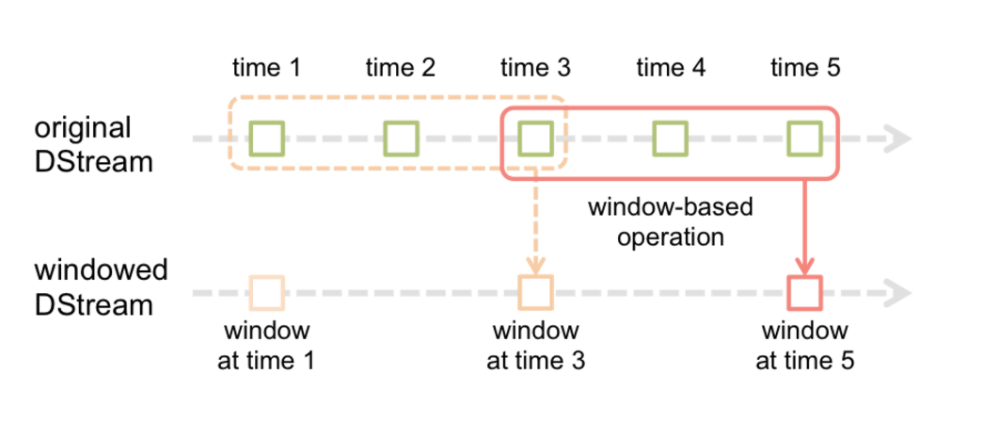
\includegraphics[scale=0.5]{one.png}

When applying the machine learning algorithms, the data is sent in batches through the function, each updating the model slightly to fit the data better. 


\subsection{Applying Spark Streaming to Kmeans} 

The data arrives in a stream, so the clusters are estimated dynamically and updated as data arrives. If nt  of points already assigned to the cluster and mt  are the number of points added to the cluster in the given batch, then nt+1= nt + mt  . If ct  is the previous center of the cluster and alpha is the number of decay, or forgetfulness of the estimates, then ct+1 = (ctnta+xtmt)/(nta+mt)

This means that as new data arrives through the stream, the clusters are adjusted and certain data points are forgotten. The decay rate uses a half life parameter, which can be adjusted through the code

\begin{verbatim}
ssc = StreamingContext(sc, 1)

lines1 = ssc.textFileStream("file:///mnt/vdatanodea/
		datasets/creditcards/credit/b")
        
trainingData = lines1.map(lambda line: 
		Vectors.dense([float(x) for x in 
    	line.strip().split(' ')])).cache()
trainingData.pprint()

lines2 = ssc.textFileStream("file:///mnt/vdatanodea/
datasets/creditcards/credit/c")

testData = lines2.map(lambda line: 
	LabeledPoint( float(line.split(" ")[1]), 
	Vectors.dense(line.split(" ") [0])) )
testData.pprint()

model = StreamingKMeans(k=2, 
	decayFactor=1.0).setRandomCenters(2, 1.0, 0)

model.trainOn(trainingData)
ssc.start()
\end{verbatim}

While this can be used to train the data, spark streaming is far more useful when it comes to predicting data since it can take live data and calculate the risk of fraud with every purchase. 


\section{Spark Streams to test Data}

Spark streaming can take a text file, use map to clean up the data int the right format, and then make it a stream. After doing this for both the training and text data, we can use the transform function t turn it int a list of RDD objects. Then, for each RDD object, it can predict the data, check it since it is test data, and get the average error value.

\begin {verbatim}
sc = SparkContext(conf = conf)

ssc = StreamingContext(sc, 1)
lines1 = ssc.textFileStream("file:///mnt/vdatanodea/
	datasets/creditcards/credit/b")
trainingData = lines1.map(lambda line: 
	LabeledPoint( float(line.split(" ")[1]), 
    [(line.split(" ") [0]),
    (line.split(" ") [2])])).cache()
trainingData.pprint()

lines2 = ssc.textFileStream("file:///mnt/vdatanodea/
	datasets/creditcards/credit/c")
testData = lines2.map(lambda line: LabeledPoint
	(float(line.split(" ")[1]), [(line.split(" ")[0])
    	, (line.split(" ") [2]) ])).cache()
testData.pprint()

def handle_rdd(rdd):
    count = 0
    total = 0
    
    for r in rdd.collect():
        print( r.map(lambda p: (p.label, 
        	p.features, lr.predict(p.features))) )
        total = x.filter(lambda d: d[0] != d[1]).count()
        	/ float(testData.count())
        count += 1
        
    print(total/count)
    
labelsAndPreds = 
		testData.transform(lambda rdd: handle_rdd)

labelsAndPreds.pprint()
ssc.start() 
\end{verbatim}

Ideally though, it spark streaming should be used to predict live data, allowing users to immediately tag potential credit card fraud and address it in a timely fashion. The real world applications for spark streaming give it a huge advantage in the real world. The only disadvantage though is that you cant do functions like sort since you only have access to a certain portion of the dataset at a given time. So depending on the type of computation needed, it can be may or may not be useful. When it comes to detecting credit card fraud in real time though, it can be extremely useful.  

\section{Analysis}
We did two levels of analysis: comparing different machine learning algorithms to train credit card fraud data and comparing Spark vs Spark Streaming. We compared Linear Support Vector Machine, Logistic Regression, K-means, Random Forest, and Gradient Boosted Trees via the test error value, summarized in the table below:

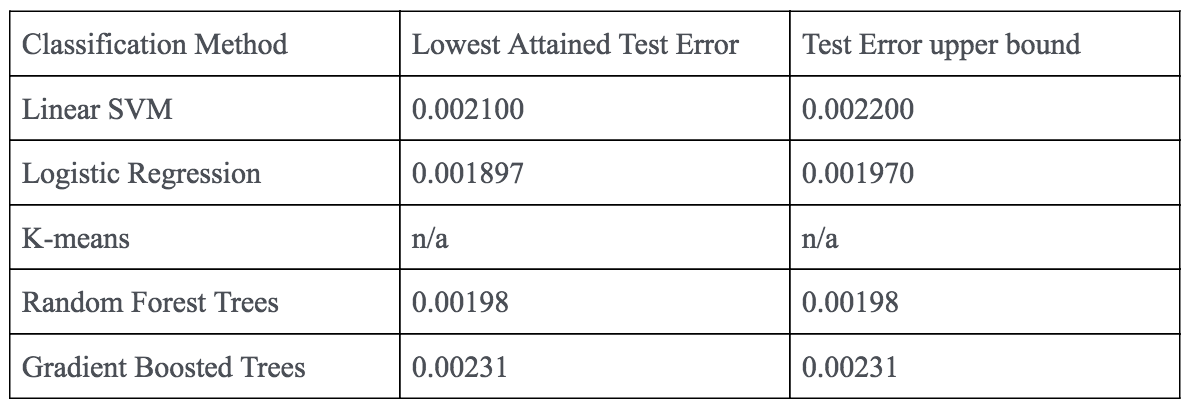
\includegraphics[scale=0.4]{three.png}

Upon initial review, it is apparent that the error in all our models are all very low, as the maximum test error can be is 1.0 (all of the predicted values are wrong). This may be due to the imbalanced nature of our data: the model is able to predict accurately because it has seen a lot of non-fraudulent transactions, which are the bulk of our test dataset. The error seems to originate from predicting fraudulent behavior, as it does not have a relatively high exposure to such data points. 

In further examination, it is apparent that preferred models for our dataset are, in order of decreasing accuracy, Logistic Regression, Random Forest Trees, Linear SVM, and Gradient Boosted Trees. Our reasoning for such behavior is that Gradient Boosted trees tends to overfit data as a result of the use of shorter decision trees with high bias and low variance. Thus, we suspect that the imbalance in our data contributed largely to overfitting of the model.

Linear SVM’s error rate was surprisingly high, but because Linear SVM tries to maximize the distance between the two classes of data, the error came from the data points sitting on the decision boundary, which makes sense as we only accounted for how many times the card was used and the amount of money spent rather than including more features that would have helped our classes of data account for more variety. 

It is not a surprise that Logistic Regression and Random Forest Trees performed most competitively, as Random Forest Trees is widely popular for its accuracy and reliability. Its excellent performance was most likely due to its usage of deeper, unpruned decision trees, versus Gradient Boosted Trees’ shorter trees. Logistic Regression does not run in O(n) time, unlike K-means (which could not produce a test error) but produces a more accurate and consistent model. 

Analyzing Spark vs Spark Streaming turned out to be much more difficult than expected, as producing test error is not straightforward. Additionally, Spark Streaming is much better for live streams of data without correct labels, unlike our own. This would make it extremely useful in real world analysis of credit card data, and is versatile as it is possible to run the same machine learning algorithms we tested in Spark. In such a case, we would be able to compare Spark and Spark Streaming more directly, which is a possible avenue for future research (or will be accomplished in the next week). 

\section{Conclusion}

Through this exploration of many Spark mllib classifiers and Spark Streaming, we were able to find the most effective model for our dataset of credit card data, which is more or less representative of all anonymized credit card data. Our analysis and conclusions tied together the fundamental concepts of each model with our observed results, allowing us a deeper understanding of each model and an intuition of the pipeline process for Spark and Spark Streaming. Usages of this research include further credit card data research and learning about other imbalanced datasets, live or static, applicable to the current intersection of data science and machine learning at large. 

\section{Sources}

1. "Spark Overview." Overview - Spark 2.1.0 Documentation. N.p., n.d. Web. 13 Apr. 2017.

2. McDonald, Carol. "Real Time Credit Card Fraud Detection with Apache Spark and Event Streaming." Real Time Credit Card Fraud Detection with Apache Spark and Event Streaming | MapR. MAPR, 3 May 2016. Web. 30 Mar. 2017. <https://mapr.com/blog/real-time-credit-card-fraud-detection-apache-spark-and-event-streaming/>.

3. Vogiatzis, Michael. "Using Spark for Anomaly (Fraud) Detection." Michael Vogiatzis. N.p., 21 May 2016. Web. 30 Mar. 2017. <https://micvog.com/2016/05/21/using-spark-for-anomaly-fraud-detection/>.

4."Linear Methods - RDD-based API." Linear Methods - RDD-based API - Spark 2.0.2 Documentation. Apache, n.d. Web. 13 Apr. 2017. <https://spark.apache.org/docs/2.0.2/mllib-linear-methods.htmllinear-support-vector-machines-svms>.

"Linear Methods - RDD-based API." Linear Methods - RDD-based API - Spark 2.0.2 Documentation. Apache, n.d. Web. 13 Apr. 2017. <https://spark.apache.org/docs/2.0.2/mllib-linear-methods.htmllogistic-regression>.


5. "Linear Methods - RDD-based API." Linear Methods - RDD-based API - Spark 2.0.2 Documentation. Apache, n.d. Web. 13 Apr. 2017. <https://spark.apache.org/docs/2.0.2/mllib-linear-methods.htmllogistic-regression>.



\end{document}